% !TeX root = ../../main.tex
\section{Hydraulic wash column design}\label{section: hydraulic wash column}

 Initially, three types of wash column had been considered: gravity, hydraulic, and mechanical. The main disadvantage with using gravity wash column is the long residence time, which can last as long as several hours, while hydraulic and mechanical wash columns have residence time of 10 to 15 minutes. Both hydraulic and mechanical wash columns are subject to compressive force and pressure drop. Due to the use of moving mechanical parts in the mechanical wash column, it was considered a less desirable choice for this process. Hydraulic wash column has been deemed the most suitable. This is a technique that combines continuous solid-liquid separation with counter-current washing. 

\subsection{Steady state model}   

Typically, the design of a hydraulic wash column should be based on pilot-scale experiments to determine appropriate dimensions at varying operating conditions. In this design, a model from van Oord-Knol \cite{van_oord-knol_hydraulic_2000} has been used for modelling the steady-state performance of the column. The hydraulic wash column has been modelled based on volume and force balances using initial dimensions provided by van Oord-Knol \cite{oordknol_dynamic_2002}. The aim of the modelling was to determine an appropriate steer flow rate, feasible column diameter, and the values of pressure at different sections of the wash column for attaining a 99.9 \% pure PNT product flow.  

% Typically, the design of a hydraulic wash column should be based on pilot-scale experiments to determine appropriate dimensions at varying operating conditions. In this design, a model from van Oord-Knol \cite{van_oord-knol_hydraulic_2000} has been used for modelling the steady-state performance of the column. The hydraulic wash column has been modelled based on volume and force balances using initial dimensions provided by van Oord-Knol \cite{oordknol_dynamic_2002}. Some variables were used to observe the performance of the column. The aim of this model was to determine an appropriate steer flow rate, feasible column diameter and determine the pressure at different sections of the wash column in  order to attain a 99.9 \% pure PNT product flow.  

Purification in the hydraulic wash column occurs through displacement and crystallisation of wash liquid on the crystals. TNO had developed a hydraulic wash column with recovery greater than 99.9\% \cite{noauthor_melt_nodate}. Based on this, the model assumes 99.9 \% solid-liquid separation in the wash column with negligible amount of liquid in the product flow and the wash front. However, if impurities are entrapped in the crystal lattice during crystallisation, these will not be removed and would be present in the product stream as impurity. This highlights a disadvantage of hydraulic wash column compared to gravity wash column, for gravity wash column allows some impurities to be removed from the crystals during the long residence time \cite{van_oord-knol_hydraulic_2000}.

\begin{wrapfigure}{R}{0.5\linewidth}
\centering
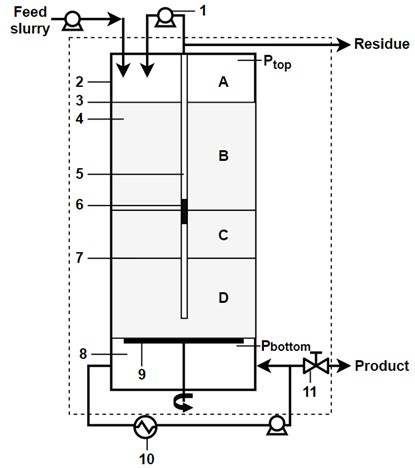
\includegraphics[width=0.4\textwidth]{chapters/3-separation/figures/hydraulic.jpg}
\caption{A schematic diagram of the hydraulic wash column: 1) steer flow pump 2) column wall 3) bed level 4) packed bed 5) filter tube 6) filter 7) wash front level 8) reslurry section 9) rotating knife 10) melter 11) product flow valve; A) slurry section B) filtration section C) stagnant section D) wash front section \cite{van_oord-knol_hydraulic_2000}}
\label{fig:hydraulic}
\end{wrapfigure}

Figure \ref{fig:hydraulic} illustrates the characteristics of the hydraulic wash column and the components required during operation. The feed slurry contains a mixture of the solid PNT crystals and the mother liquor consisting of MNT, the trace amount of ONT, and the remaining PNT that has not crystallised from the MSMPR crystalliser. The feed enters the column into the slurry section. Due to difference in density, the solid crystals will fall down the column and sediment. As the crystals move down the column, they form a packed bed of solid. The filter in the filter tubes removes the mother liquor from the filtration section. A part of the mother liquor gets recycled back into the column by the steer pump, known as the steer flow, and some mother liquor is purged out as residue or waste. The pressure drop across the filter drives the solids down the column and the mother liquor up through the filter tubes. This is where solid-liquid separation takes place. The solid crystals form a densely packed moving bed in the wash front section with no mother liquor present. The rotating knife at the bottom will scrape the bottom of the packed bed, so that pure PNT solids fall into the bottom section. The melter at the bottom melts the PNT solids. Some of the molten solid gets pumped out as the product stream through the outlet valve, and some PNT gets recycled back into the bottom section. Due to the pressure drop at the valve, the washing liquid gets pushed up into the washing section of the column where counter current washing occurs. The solid crystals, which are at a lower temperature, causes the washing liquid to crystallise on the solid particles, leading to a frozen wash front level. This counter current washing allows for 99.9 \% ultrapurification. 

\subsubsection{Volume balance} 
The model has been based on the assumption that the liquid and solid in the system were incompressible. For simplicity, density and viscosity have been assumed to be independent of temperature. Thus, volume balance can be performed and will function like the mass balance. 

The overall volume balance at the top section is

\begin{equation}
\phi_{\mathrm{feed}}+\phi_{\mathrm{steer}}=\phi_{s,\mathrm{filters}}+\phi_{ml.\mathrm{filters}}
\end{equation}

\noindent where $\phi_{\mathrm{feed}} (m^{3}/s)$ is the feed flow rate, $\phi_{\mathrm{steer}} (m^{3}/s)$ is the steering flow, $\phi_{\mathrm{s,filters}} (m^{3}/s)$ is the crystal flow at the filters and $\phi_{\mathrm{ml,filters}} (m^{3}/s)$ is the mother liquor flow at the top section.

The total length of the top section remains constant. The length of the filtration section $ L_{\mathrm{filtration}} (m)$,  was derived from the solid balance in the top section where $\alpha_1 (m^3/m^3)$ is the crystal fraction in the feed slurry, $\alpha_2 (m^3/m^3)$ is the crystal fraction in the slurry section, $\epsilon$ is the porosity in the filtration and stagnant section and $A_c (m^2)$ is the cross sectional area of the wash column. 

\begin{equation}
\frac{\dd L_{\mathrm{filtration}}}{\dd t} = \frac{1}{A_c(1-\alpha_2-\epsilon)}(\alpha_1\phi_{\mathrm{feed}}-\phi_{s,\mathrm{filters}})
\end{equation}

In the bottom section, there is the stagnant zone with the crystals. Then there is the wash zone with only the crystal and the wash liquid at steady state. The wash liquid crystallises due to low temperature at the wash front. The crystallisation of the wash liquid can be related to the disappearance of the wash liquid by difference in density of the solid and liquid.$C_s (m^3/s)$ is the solidification rate of wash liquid to solid at the wash front, $C_l (m^3/s)$ is the solidification rate at the wash front solid to liquid. 
\begin{equation}
C_l= \frac{\rho_s}{\rho_l}C_s
\end{equation}

The amount of crystallised material was calculated based on a heat balance and temperature difference between the feed and the melt. This assumes the total cooling capacity of the crystals is used to crystallise the wash liquid.$c_p (kJ/kgK)$ is the specific heat capacity, $T_{\mathrm{melt}} (K)$ is the melting temperature, $T_{\mathrm{feed}} (K)$ is the feed temperature and $\Delta H_m (kJ/kg)$ is the heat of fusion. 
\begin{equation}
C_s= \frac{c_p(T_{\mathrm{melt}}-T_{\mathrm{feed}})}{\Delta H_m}Q_{s,\mathrm{filters}}
\end{equation}

The length of the wash section is related to the wash-liquid flow entering the knife and the wash liquid that crystallises. This assumes wash liquid is not lost through the filters which is ensured by positioning the filters above the wash section.$\epsilon_w$ is the porosity in the wash section


\begin{equation}
\epsilon_w A_c \frac{\dd L_{\mathrm{wash}}}{\dd t}= \phi_{wl,\mathrm{knife}}-C_l
\end{equation}

The wash column during operation forms 3 layers of filtration, stagnant and wash sections. Within the filtration and stagnant section it is assumed the porosity and permeability remain constant. Since the crystals form a densely packed column $\epsilon$ was approximated at 0.45 \cite{jansens_furification_1995}. Due to the wash-liquid crystallisation at the wash zone an abrupt change in porosity and permeability was considered. The consolidation of the crystal bed were neglected in this model, however under compressive force from the pressure at the top section this may not be a valid assumption and will have to be explored further through experiments. The porosity in the wash zone was calculated from the equation below. 

\begin{equation}
\epsilon_{w}= \epsilon-(1-\epsilon)\left(\frac{c_p(T_{\mathrm{melt}}-T_{\mathrm{feed}})}{\Delta H_m}\right)
\end{equation}

At steady state, the wash section is constant with no flow of mother liquor into or out of the bottom section. The mother liquor at the top section leaves the column through the filter and splits into residual and steer flow. 
\begin{equation}
\phi_{\mathrm{residue}}= \phi_{ml,\mathrm{filters}} - \phi_{\mathrm{steer}}
\end{equation}

The volume balance at the melting circuit is based on the assumption that crystals are molten the moment they enter the melting circuit. The wash liquid enters the column at the melting temperature. 
\begin{equation}
\frac{\rho_s}{\rho_l}\phi_{s,\mathrm{knife}}= \phi_{wl,\mathrm{knife}} - \phi_{\mathrm{product}}
\end{equation}


\subsubsection{Force balance}
The liquid pressure drop across each section were calculated with the following modified Darcy's law equation. 
\begin{align}
    \frac{\Delta P_{l,\mathrm{filtration}}}{L_{\mathrm{filtration}}} &= \frac{\epsilon \eta_{l}}{B_{\mathrm{filtration}}}\left(\frac{\phi_{ml,\mathrm{filters}}}{\epsilon A_c} - \frac{\phi_{s,\mathrm{filters}}}{1-\epsilon A_c}\right) \\
    \frac{\Delta P_{l,\mathrm{stagnant}}}{L_{\mathrm{stagnant}}} &= \frac{\epsilon \eta_{l}}{B_{\mathrm{stagnant}}}\left(-\frac{\phi_{ml,\mathrm{bottom}}}{\epsilon A_c} - \frac{\phi_{s,\mathrm{filters}}}{1-\epsilon A_c}\right) \\
    \frac{\Delta P_{l,\mathrm{wash}}}{L_{\mathrm{wash}}} &= \frac{\epsilon \eta_{l}}{B_{\mathrm{wash}}}\left(-\frac{\phi_{wl,\mathrm{knife}}}{\epsilon_w A_c} - \frac{\phi_{s,\mathrm{knife}}}{1-\epsilon_w A_c}\right)
\end{align}

The liquid pressure gradient at each section were assumed to be constant since the packed bed is considered incompressible. The liquid pressure at the top in the slurry section was based on the pressure at the filter and the pressure drop over the filtration section. 
\begin{equation}
P_{\mathrm{top}} = P_{\mathrm{filters}} + \Delta P_{l,\mathrm{filtration}}
\end{equation}

The pressure at the bottom is equal to the pressure drop in the valve of the melting circuit. This pressure drop across the valve is determined through a linear relation with the product flow rate.
\begin{equation}
P_{\mathrm{bottom}}=\Delta P_{\mathrm{valve}} = K_w\phi_{\mathrm{product}}
\end{equation}

The pressure in the melting circuit was calculated using the equation below. 
\begin{equation}
\Delta P_{\mathrm{valve}} = \Delta P_{l,\mathrm{stagnant}} + \Delta P_{l,\mathrm{wash}} + P_{\mathrm{filters}}
\end{equation}

\subsection{Modelling results}
The linear system of algebraic equations from the steady state model were solved using input variables and parameters shown in Table \ref{tab:inputsparameters}. 

\begin{table}[h]
\centering
\caption{Input variables and parameters}
\label{tab:inputsparameters}
\begin{tabular}{lS[table-format=1.2e2]s|lS[table-format=1.2e2]s}
\toprule
\multicolumn{3}{c|}{\textbf{Inputs}}                     & \multicolumn{3}{c}{\textbf{Parameters}}          \\ \midrule
$\phi_{\mathrm{feed}}$  & 4.27e5 & \cubic\m\per\s        & $\epsilon$                & 0.45     &           \\
$\phi_{\mathrm{steer}}$ & 2.65e5 & \cubic\m\per\s        & $\mathrm{B_{filtration}}$ & 1.37e-13 & \square\m \\
$\alpha_1$              & 0.906  & v/v                   & $\mathrm{B_{wash}}$       & 1.01e-13 & \square\m \\
$\mathrm{K_{w}}$        & 1.9e10 & \pascal\s\per\cubic\m &                           &          &           \\ \bottomrule
\end{tabular}
\end{table}

During operation of the hydraulic column  variations in the length of the filtration, stagnant and wash section is possible. Therefore, simulations of variable filtration and wash section lengths were implemented on Excel to determine the effect on pressures at different sections of the column. With proper controls in place, the sections should not vary significantly during normal operation, therefore variation in filtration and wash section would be designed to be between 0.27 to 0.30 m.  
\begin{wrapfigure}{R}{0.5\linewidth}
\centering
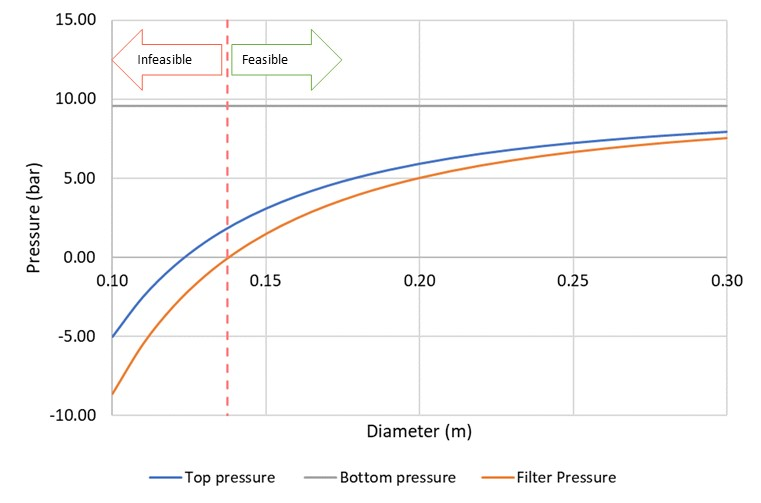
\includegraphics[width=\linewidth]{chapters/3-separation/figures/diameter.jpg}
\caption{Effect of varying diameter}
\label{fig:dia_col}
\end{wrapfigure}

The length of the column was fixed at 0.8 m. The diameter of the column was varied from 0.1 m to 0.3 m to observe the impact it has on the pressure across the column. Figure \ref{fig:dia_col} indicates when the diameter is less than 0.165 m the model suggests negative pressure at the filter which could imply instead of mother liquor flowing upwards through the filter tube, it could be flowing in the reverse direction. The pressure at the top is also negative indicating at these conditions the fluid flow in the column may not be in the desirable downward direction. A suitable diameter was chosen at 0.17 m allowing for slight variations in the section lengths over time under normal operation.

\begin{wrapfigure}{R}{0.5\linewidth}
\centering
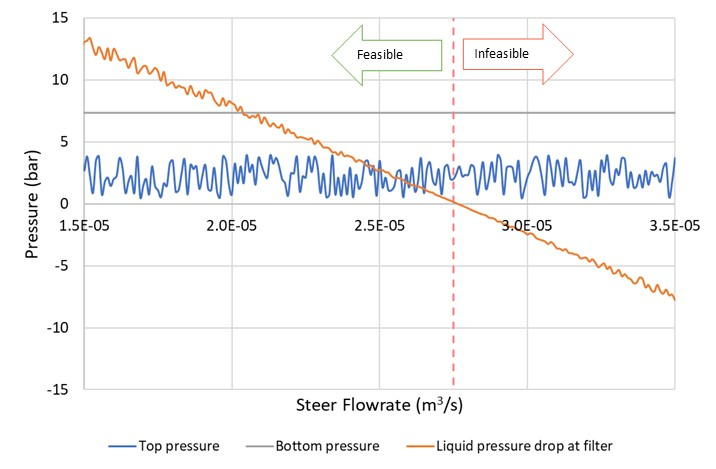
\includegraphics[width=\linewidth]{chapters/3-separation/figures/steerflow.jpg}
\caption{Effect of varying steer flow rate}
\label{fig:steer_col}
\end{wrapfigure}

Steer flow is the flow rate of the mother liquor being recycled back into the column from the filter tubes whilst some mother liquor are removed as residual flow. The filtrate being recycled back into the column increases the transport force. Steer flowrate was varied from $1.5 \times 1o^{-5}$ to $3.5 \times 1o^{-5}$ $m^{3}/s$. Figure \ref{fig:steer_col} shows the unfeasible and feasible region of operation. Above a steer flow rate of $2.7 \times 1o^{-5}$ $m^{3}/s$, the model shows negative liquid pressure drop at the filter. However, at lower steer flow such as $1.5 \times 1o^{-5}$ $m^{3}/s$ the filter pressure increases significantly to more than 10 bar. In order to attain a lower pressure but also ensure the column is operating in a feasible region, the steer flow rate at $2.65 \times 1o^{-5}$ $m^{3}/s$ was chosen. At this flow rate there is an allowance for variation in the flowrate whilst the column is still operating in the feasible region. The steer flow appears to have no impact on the bottom pressure. This is because the bottom pressure mainly relies on the valve resistance coefficient. 

\begin{wrapfigure}{R}{0.5\linewidth}
\centering
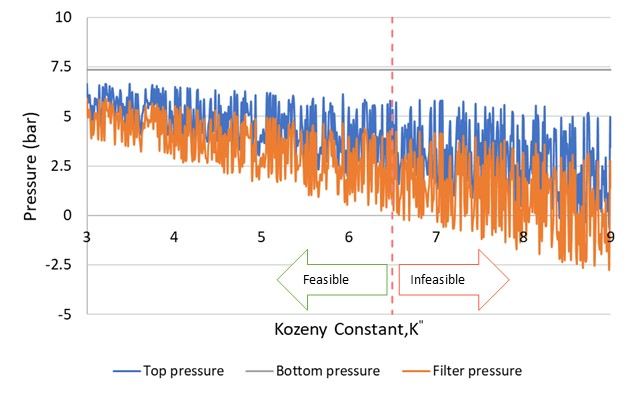
\includegraphics[width=\linewidth]{chapters/3-separation/figures/kozeny.jpg}
\caption{Effect of varying Kozeny constant}
\label{fig:koz_col}
\end{wrapfigure}

The permeability constant, B, was determined using Kozeny constant, K".  In this process, K" was considered to be 5, assuming the crystal is spherical. A sensitivity analysis on the permeability constant was conducted by varying K".Figure \ref{fig:koz_col} shows when K">6.5, the design becomes infeasible reaching negative filter pressures.The sensitivity analysis was conducted with the filtration and wash section varying between 0.27 and 0.3 m to observe the range of pressure in the column. It is evident, the hydraulic column is sensitive to the Kozenzy constant and the permeability of the packed bed. This was expected due to the inverse relationship between the permeability constant and pressure drop in the modified Darcy's law equation. It is essential to conduct pilot-scale experiments to obtain more accurate value for K" and the permeability constant to get a reliable observation of the column's performance. 

Based on literature \cite{jansens_furification_1995} the temperature profile at the wash front was found to be independent of the axial and radial position in the column if the distance of the wash front from the filter is greater than 0.1 m. In this design the filter tube was positioned 0.1 m above the wash front. The temperature profile was also found to be independent of the product throughput. Additionally, compressive stress impacts the permeability of the bed and causes deformation of the crystal particles. In this process the crystals are melted; the crystal particle size or shape were not of concern so compressive stress was not considered further. 

\begin{table}[h]
\centering
\caption{Stream table for the hydraulic wash column.}
\label{tab:wash column stream table}
\begin{tabular}{@{}l|l|l|l|l|l|l|l|l|l@{}}
\toprule
Stream            & 3-01 & 3-02 & 3-03 & 3-04 & 3-05 & 3-06 & 3-07 & 3-08 & 3-09 \\ \midrule
Temperature (K)   & 280 & 324 & 324 & 324 & 324 & 280 & 280 & 280 & 324 \\ \midrule
Pressure (atm)    & 1   & 1   & 1   & 1   & 1   & 1   & 1   & 1   & 1 \\ \midrule
Phase & \begin{tabular}[c]{@{}l@{}}Solid \\ + liquid \end{tabular}  & \begin{tabular}[c]{@{}l@{}}Solid \\ + liquid \end{tabular} & Liquid & Liquid & Liquid & Liquid & Liquid & Liquid & Liquid \\ \midrule
Liquid fraction &  0.1995 &  0.1995 & 1 & 1 & 1 & 1 & 1 & 1 & 1\\ \midrule
Solid fraction  &  0.8005  &  0.8005 & 0 & 0 & 0 & 0 & 0 & 0 & 0 \\ \midrule
MNT (kmol/day)  &  2.72 & 0.00 & 0.00 & 0.00 & 0.00 & 10.55 & 10.55 & 2.72 & 0.00 \\ \midrule
ONT (kmol/day)  &  0.17 & 0.00 & 0.00 & 0.00 & 0.00 & 0.67 & 0.67 & 0.17 & 0.00 \\ \midrule
PNT (kmol/day)  &  21.99 & 22.48 & 22.48 & 2.58 & 19.90 & 8.12 & 8.12 & 2.09 & 19.90\\ \bottomrule
\end{tabular}
\end{table}

\subsection{Physical design}
Like the physical design for the crystalliser in Section \ref{sec:physical design crystalliser}, the hydraulic wash column vessel has been designed in accordance with British Standards and also to consist of a cylindrical shell and two ellipsoidal domed ends. From \textbf{BS5500: 1997}, the minimum thickness for a cylindrical shell, $e_{\mathrm{cyl}}$, can be computed as 

\begin{equation}
    e_{\mathrm{cyl}} = \frac{p D_i}{2f - p}
\end{equation}

\noindent where $p$ is the design pressure of the vessel, and $D_i$ is the internal diameter of the vessel taken to be the same as $D$ as defined in Section \ref{sec: crystalliser mass balance}. For a vessel with ellipsoidal ends, the minimum thickness, $e_{\mathrm{end}}$, can be calculated using the methodology outlined in Section 3.5.2 of \textbf{BS5500: 1997}. The values of $e_{\mathrm{cyl}}$ and $e_{\mathrm{end}}$ have been obtained as 0.36 mm and 0.918 mm. After a corrosion factor of 1.5 mm has been taken into account, a uniform wall thickness of 3 mm has been chosen for both the shell and the dome ends. 

Eight ports are required in total, namely: the vessel inlet at the top, the top recycle, the filter tube outlet, the vessel outlet at the bottom, the bottom recycle, a safety relief valve, and two sightholes. Pipes with nominal pipe size (NPS) of 1/2 inch have been selected for all ports except the two sightholes on the wash column. For the two sightholes, 2 inch pipes have been used instead. 

Four filter tubes 680 mm in length, 20 mm in diameter, and 3 mm in wall thickness have been implemented in the design. A set of four knives have been implemented at the bottom of the vessel. Support structures are not included in the design but are nonetheless recommended for implementation to secure the position of the vessel due to the inherent imbalance of weights. The operators are recommended to select support structures appropriate to their circumstances. 

\begin{table}[h] \label{tab:wash column mech design summary}
\centering
\caption{Summary of key physical design parameters for the hydraulic wash column.}
\begin{tabular}{@{}l|l@{}}
\toprule
\textbf{Inner diameter (mm)}                &    170.00 \\ \midrule
\textbf{Height of cylindrical shell (mm)}   & 800.00 \\ \midrule
\textbf{Crown radius (mm)}                  & 136.00 \\ \midrule
\textbf{Knuckle radius (mm)}                & 24.82  \\ \midrule
\textbf{NPS of sightholes (inch)}                & 2 \\ \midrule
\textbf{NPS of all other ports (inch)}                & 1/2 \\ \midrule
\textbf{Flange class}                       & 300 \\ \midrule
\textbf{Knife length (mm)}              & 156.00 \\ \midrule
\textbf{Number of knives}            & 4 \\ \midrule
\textbf{Knife width (mm)}          & 6.5 \\ \bottomrule
\end{tabular}
\end{table}

\begin{figure}[h]
    \centering
    \includesvg[scale=0.3,inkscapelatex=false]{figures/Wash_column_schematic.svg}
    \caption{Schematics for the hydraulic wash column: (a) perspective (b) right-side section (c) front section (d) section for detailed view of knives (e) section for detailed view of filter tubes crossing.}
    \label{fig:wash column schematic}
\end{figure}

\newpage
\begin{figure}[h!]
    \centering
    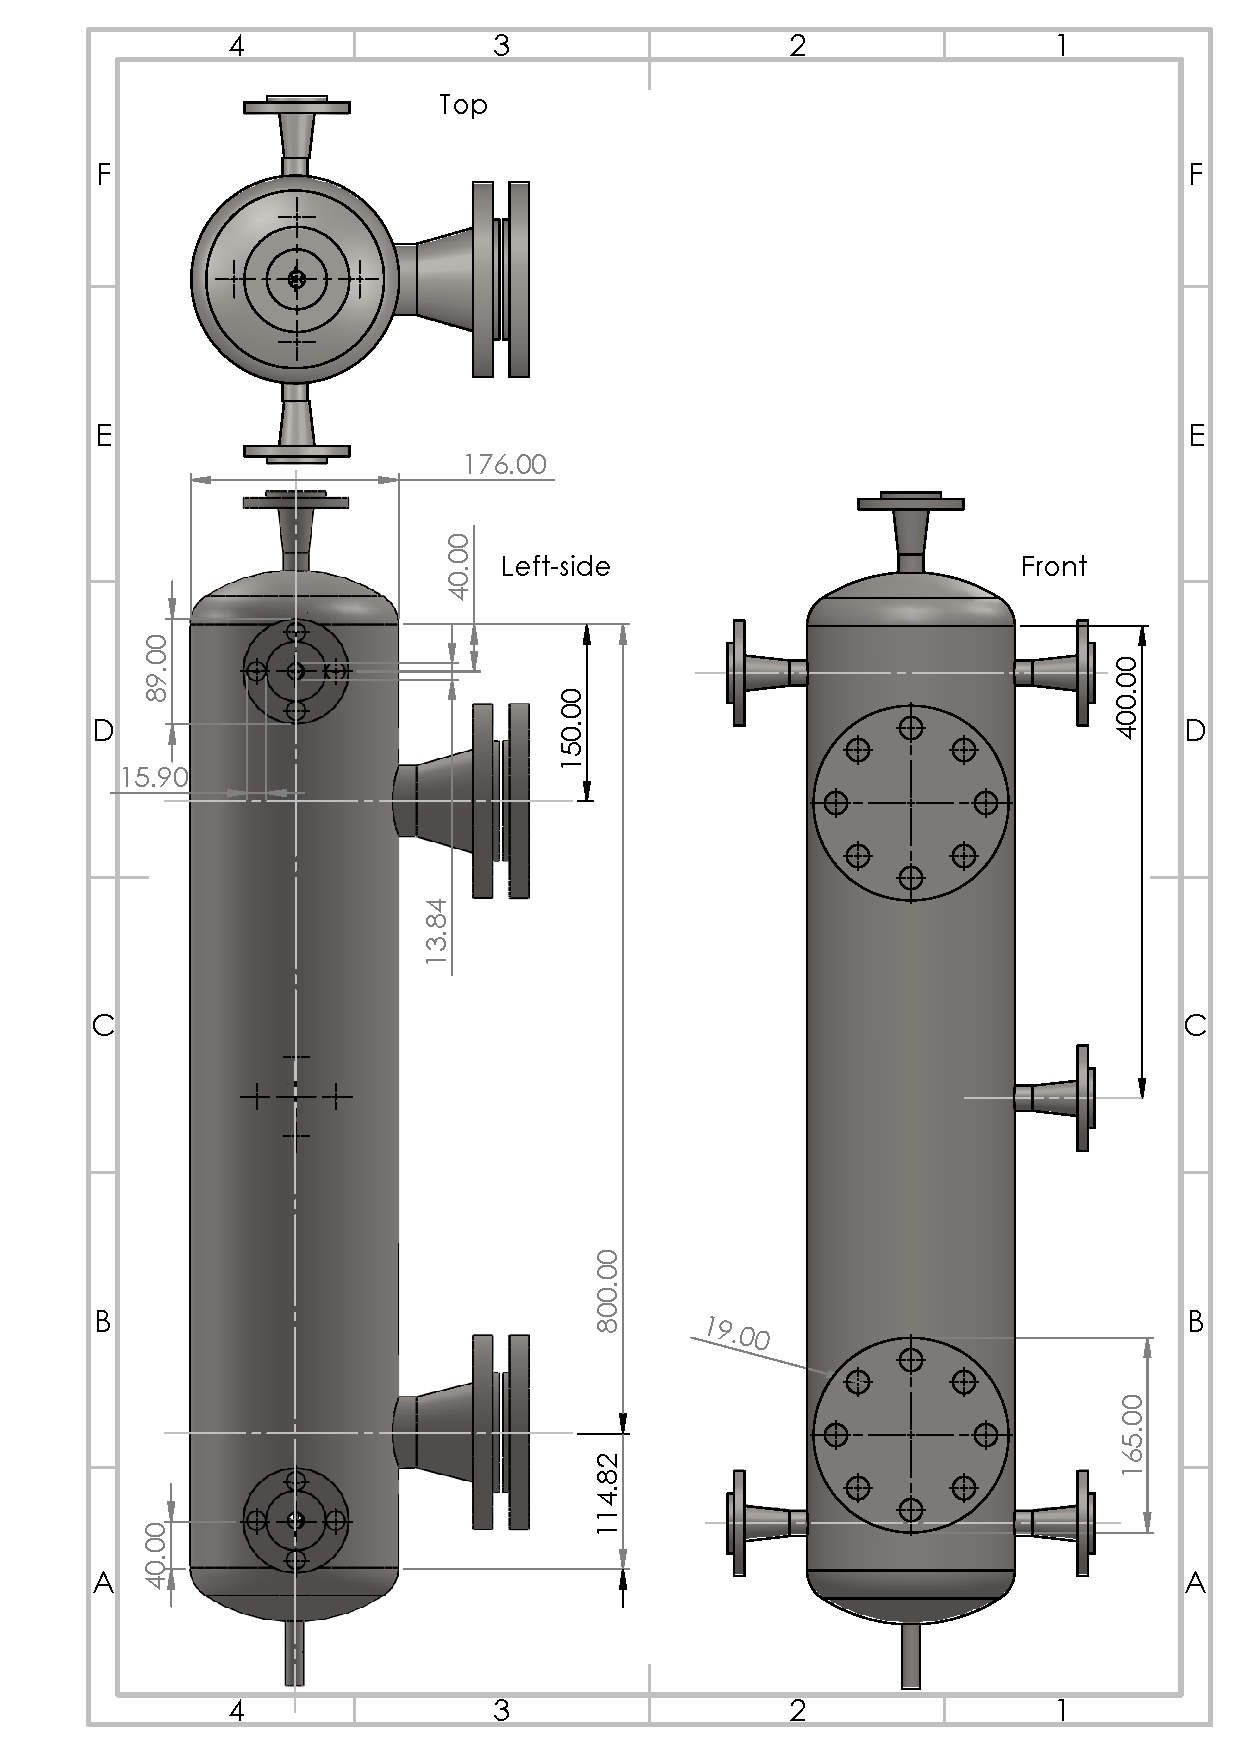
\includegraphics[scale=0.8]{chapters/3-separation/figures/Hydraulic_Wash_Column_GA.PDF}
    \caption{GA drawing for the hydraulic wash column}
    \label{fig:wash column GA}
\end{figure} 

\newpage

\subsection{Conclusion and Recommendations}

Crystallisation was used in this separation due the large difference in melting temperatures of the nitro toluene isomers (mainly para and meta) and the requirement for a high purity, high recovery separation step. The crystallisation gave a 90.6\% recovery of PNT solids from the liquid feed mixture. 



On the issue of fouling, removal mechanisms such as mechanical devices (hammers, scrapers) or chemical removal like the introduction of a solution to dissolve the encrusted layer. Preferably, the removal would be on line to not incur shutdown costs and reduce production, but if necessary, off line techniques could be used.
Moving forward, pilot studies can be carried out to determine accurate coefficients for crystallisation in both primary and secondary nucleation rather than using the approximate values for similar systems. 




